%!TEX root = ../dissertation.tex
\section{Application to Schizophrenia and Bipolar Disorder}
A comprehensive structural analysis of perturbations on a genome scale is hardly possible without heavy truncation of results or dimensionality reduction methods. Truncation is commonly performed by ranking perturbations by their p-values in ascending order and only regarding the highest ranked entries, which often amounts to less than ten individual transcripts. On the other hand, commonly used dimensionality reduction techniques include \ac{pca}, \ac{tsne}, and clustering/stratification approaches. While truncation enables human-readable presentation of results, in principle it does not lend itself to complex polygenic events such as neurologic disease. Common dimensionality reduction techniques are useful in providing structural overview of a high-dimensional dataset, but give little insight into causal relationships of single entities. We thus aimed to find an alternative approach to dimensionality reduction which conserves the internal relationships inherent to the data, and which profits from the network organisation of our input data.

For the application of \emph{miRNeo} data to real-world problems, suitable psychiatric and neurologic disease datasets were sought in the common repositories ArrayExpress, NCBI GEO, and Synapse. Among the datasets with agreeable quality, \ac{scz} and \ac{bd} were the only diseases with sample amounts that allowed a statistically valid analysis of sexual dimorphisms. While many neurologic disease studies are simply limited in their number of subjects, autism presented a different issue: the majority of donors were males (more than 90\%). Direct analysis of miRNA expression patterns was not possible, because very few studies study miRNAs directly, yet. Thus, studies on mRNA were substituted to infer on miRNA dynamics.

\begin{method}

\subsection{Analysed Datasets}
Twelve datasets including 1361 subjects were downloaded from their repositories (Table \ref{tab:datasets}). 
Data of DLPFC \ac{seq} of 579 SCZ patients and controls was obtained from the Common Mind Consortium (\url{http://www.synapse.org/CMC}). To address the diverse origins and technological aspects of data, care was taken to appropriately unify and normalise the data. The data preparation and meta analyses were performed essentially as described by Gandal and colleagues.\cite{Gandal2018} Samples of brain regions not consistent with the research question (e.g., cerebellum), or from patients with diseases other than SCZ or BD, were removed from datasets on a case-by-case basis. \ac{seq} datasets were used to individually confirm the perturbations found in the meta-analysis of microarray studies.

\begin{table}
\sffamily
\small
\centering
\begin{tabular}{c | c | c | c | c | c}
source & accession & publication & technology & subjects/samples & disease\\ \hline
\hline
NCBI GEO & GSE35978 & Chen \emph{et al.}\cite{Chen2013} & microarray & 150/312 & SCZ \& BD\\ \hline
NCBI GEO & GSE12649 & Iwamoto \emph{et al.}\cite{Iwamoto2005} & microarray & 102/102 & SCZ \& BD\\ \hline
NCBI GEO & GSE53987 & Lanz \emph{et al.}\cite{Lanz2015} & microarray & 76/205 & SCZ \& BD\\ \hline
NCBI GEO & GSE17612 & Maycox \emph{et al.}\cite{Maycox2009} & microarray & 51/51 & SCZ\\ \hline
NCBI GEO & GSE21138 & Narayan \emph{et al.}\cite{Narayan2008} & microarray & 30/59 & SCZ\\ \hline
NCBI GEO & GSE5392 & Ryan \emph{et al.}\cite{Ryan2006} & microarray & 82/82 & BD\\ \hline
NCBI GEO & GSE80655 & Ramaker \emph{et al.}\cite{Ramaker2017} & RNA-seq & 96/281 & SCZ \& BD\\ \hline
NCBI GEO & GSE106589 & Hoffman \emph{et al.}\cite{Hoffman2017} & RNA-seq & 94/94 & SCZ\\ \hline
NCBI GEO & GSE68559 & Webb \emph{et al.}\cite{Webb2015} & RNA-seq & 10/98 & NA\\ \hline
NCBI GEO & GSE96659 & Fontenot \emph{et al.}\cite{Fontenot2017} & RNA-seq & 5/209 & NA\\ \hline
NCBI GEO & GSE45642 & Li \emph{et al.}\cite{Li2013} & RNA-seq & 86/670 & NA\\ \hline
Synapse & CMC & Gulyás-Kovács \emph{et al.}\cite{Gulyas-Kovacs2018} & RNA-seq & 579/579 & SCZ \& BD\\ \hline
\end{tabular}
\caption{\textbf{Data Sources for Microarray and RNA-seq Analyses.}}
\label{tab:datasets}
\end{table}

\subsection{Microarray Quality Control and Data Preparation} \label{sec:cellculture:quality}
\subsubsection{Read-In and Normalisation}
Illumina datasets were read, log$_2$-transformed, and quantile-normalised using R/lumi.\cite{Du2008} Affymetrix datasets were read and RMA-normalised (log$_2$-transformed, background corrected, quantile-normalised) using R/affy.\cite{Gautier2004} Affymetrix data were additionally corrected for 3'/5' bias using the \emph{AffyRNAdeg()} function (not available for other chip manufacturers). All available biological (e.g., sex, age) and technical (e.g., batch, \ac{rin}, post-mortem interval) covariates were collected and used for the analysis. Individual correlations of case-control status $S$ with any covariate $C$ were assessed using a linear model (R/lm) with formula $C \smallsim S$; statistical significance was determined via ANOVA (R/anova). If necessary, case-control samples were balanced to eliminate significant covariate correlations with case-control status (all p > 0.05).

\subsubsection{Outliers}
Outlier removal was performed using the method proposed by Oldham, Langfelder \& Horvath.\cite{Oldham2012} Briefly, the (dis\-/)similarity matrix of samples is transformed into a signed, weighted correlation network. Network adjacency ($a$) of samples (nodes) $S_i$ and $S_j$ is defined as: $$a_{ij} = \left(\frac{cor(S_i, S_j)+1}{2}\right)^2$$

As such, the connectivity between samples can be measured by the standardised connectivity (\emph{Z.K}), which describes the strength of correlation between any given node and all other nodes in the network. As proposed by Oldham \emph{et al.}, outliers were removed if their Z-score was below the threshold of \emph{Z.K} = -2.

\subsubsection{Annotation}
To enable comparison between datasets of diverse technical origin, probes were annotated using ENSEMBL gene identifiers using R/biomaRt.\cite{Durinck2009} To maintain comparability with the analysis by Gandal \emph{et al},\cite{Gandal2018} the same version of ENSEMBL DB (v75, Feb 2014) was used. Probes were collapsed onto single genes using the \emph{collapseRows()} function of R/WGCNA,\cite{Langfelder2008} using the maximum mean signal across all probes per gene. Of note, information loss occured by multiple collapsing of probes and integration of datasets, which can only be performed using the genes common to all datasets (i.e., represented by microarray probes). The final gene set encompassed 12\,391 individual genes, with several notable cholinergic/neurokine exceptions (CHRNA7, CHRM1, LHX8, CHKB, PRIMA1, CNTF). Missing genes result from annotation deficits between different probe sets, cannot be comprehensively manually controlled on a genome scale, and cannot be re-introduced at this stage. 

\subsection{Differential Expression Meta-Analysis}
The individual experimental datasets were each corrected for covariate influences by multiple regression based on all available biological and technical covariates. Briefly, the linear regression model was solved using matrix algebra operations. In matrix form, a linear regression model of observations $Y$ (i.e., gene expression levels), independent variables $X$ (i.e., covariates), coefficients $\beta$, and error terms $\epsilon$ can be described as: $$Y = X\beta + \epsilon$$ As a consequence, the residual sums of squares can be expressed as the cross product: $$RSS = (Y - X\beta)^T(Y - X\beta)$$ Then, the coefficients $\hat{\beta}$ can be estimated by solving the derivative: $$\hat{\beta} = (X^TX)^{-1} X^TY$$ Coefficients were estimated for all relevant technical and biological covariates (e.g. post-mortem interval, RIN, sex, age) and used to regress covariate influence on gene expression levels: $$Y_{new} = Y - (X\hat{\beta})^T$$

After covariate regression, differential expression was calculated across all datasets for each disease group using a linear mixed model with a fixed effect for each study and case-control status (»group«), and a random effect for each individual subject. Computation was performed in R, using R/nlme,\cite{Pinheiro2019} with parameters $$fixed = \smallsim group + study\textrm{\sffamily\,\,\,and\,\,\,}random = \smallsim 1|subject$$

This yielded an array of log-fold changes between cases and controls for each gene and disease. To determine statistical significance, 10\,000 permutations of the mixed-model regression were performed for each use case, randomly assigning case-control status. The resulting null distributions were used to determine \ac{fdr}, with threshold for significance at 0.05. 

\subsubsection{Sex-Specific Meta-Analysis}
Samples of all datasets were split between males and females (cases as well as controls), and individually subjected to the same procedure as the sex-independent data: covariate regression, differential expression via a linear mixed model, and estimation of statistical significance via permutation testing.

\subsubsection{Transcriptome Correlation}
Correlation of disease transcriptomes was performed by using Spearman's rank correlation coefficient. Spearman's $\rho$ was determined between SCZ and BD sex-independently as well as separately in males and females.

\subsubsection{Most Diverging Genes}
Genes were ranked by their divergence between any two compared datasets, sex-independent data of SCZ and BD, and any meaningful combination of sex-dependent data in SCZ, BD, males, and females. The divergence $\updelta$ of any gene $G$ between datasets $i$ and $j$ was defined as (\emph{logFC}: log-fold change): $$\updelta = logFC(G)_i - logFC(G)_j$$

Where positive values of $\updelta$ indicate a positive bias of $G$ towards dataset $i$.

\end{method}

\subsection{Sexual Dimorphism in Schizophrenia and Bipolar Disorder}
Sex-independent correlation replicated the finding of Gandal \emph{et al},\cite{Gandal2018} with Spearman's $\rho = 0.7100$ \mbox{(p < 0.001)}. However, diverging from the established annotation of ENSEMBL v75 to later versions of the database significantly altered the correlation coefficient, leading to lower correlation in all tested cases. Comparing the sex-independent data with only male or female subjects, those also show lower general correlation between SCZ and BD: in females, correlation was $\rho = 0.6150$ (p < 0.001), in males, $\rho = 0.5783$ (p < 0.001). While it is possible that these variations are caused by structural properties of the data unrelated to sexual dimorphism, such as the loss of power due to the reduction in size, the consistently lower correlation in sex-specific subsets also may indicate an averaging effect between male and female patients, leading to a higher correlation in spite of significant sexual dimorphism.

 To address the potential differences between male and female brain transcriptomes, which may reflect the observed clinical dimorphism, we subjected the 100 most-diverging genes between any two datasets to \ac{go} enrichment analysis (Fig.\,\ref{fig:scz-bd-go}, from Lobentanzer \emph{et al.}\cite{Lobentanzer2019a}) in hopes of identifying the most discriminating molecular pathways between SCZ and BD, and afflicted males and females. Sex-independently, the most-diverging pathways between SCZ and BD principally involved mechanisms of inflammation and immunity (e.g., ‘‘acute inflammatory response,’’ p = 0.003; ‘‘cellular response to cytokine stimulus,’’ p = 0.01).

\subsubsection{Differences in Sexual Dimorphism Between SCZ and BD}
Computation of diverging pathways between males and females in each disease indicated a larger divergence between sexes in SCZ than in BD. SCZ-biased genes of males and females showed no overlapping GO terms (Fig.\,\ref{fig:scz-bd-go}\,A), but BD-biased genes of males and females showed large GO term overlap, particularly in inflammatory components (Fig.\,\ref{fig:scz-bd-go}\,B). Notably, specific components of neurokine signalling were elevated in both males (IL-6, p= 0.007) and females (JAK/STAT, p = 0.01) with BD.

\subsubsection{Overlap of Male-Biased Genes Between SCZ and BD}
Shared transcriptional properties of SCZ and BD were identifiable only in male diverging genes. While female-biased SCZ genes showed no implications in CNS processes, male-biased SCZ and BD genes overlapped in functions concerning inflammation and immunity (Fig.\,\ref{fig:scz-bd-go}\,C). Female-biased BD genes were associated with CNS function and development (Fig.\,\ref{fig:scz-bd-go}\,D).

\begin{figure}[ht]
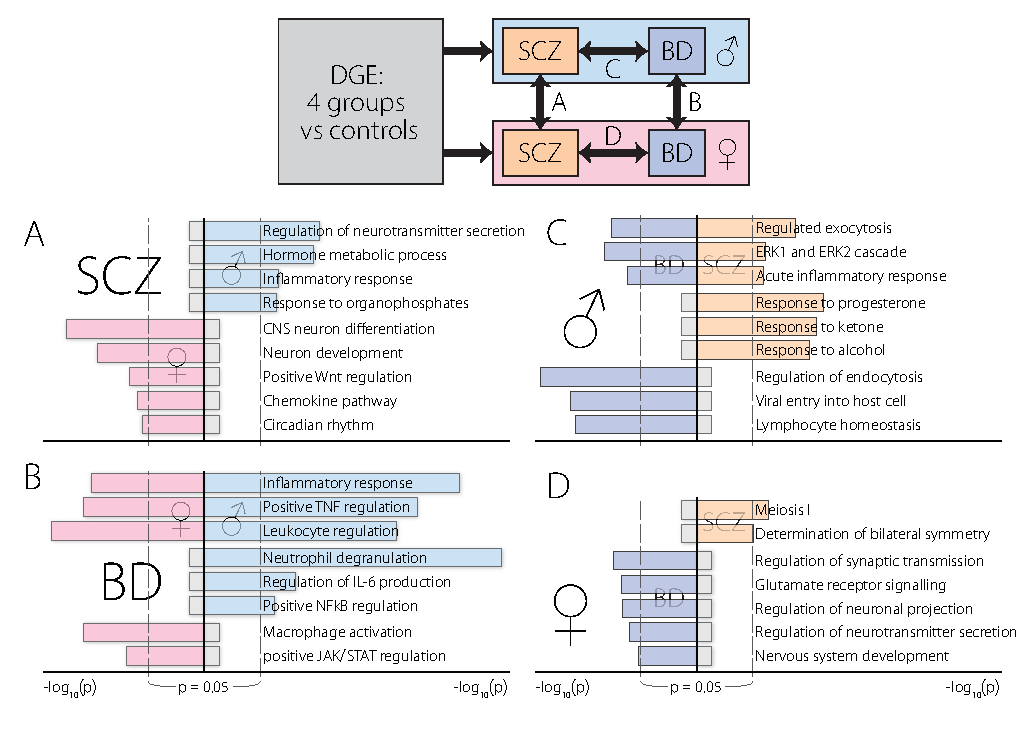
\includegraphics[width=\textwidth]{figures/scz-bd-go}
\caption[GO Enrichment of Diverging Genes.]{\textbf{GO Enrichment of Diverging Genes.} Results of differential gene expression were dually compared: SCZ versus BD and male versus female (indicated by colours). GO enrichment of the top 100 distinguishing genes in one dimension was compared with the other for each pair of combinations. \textbf{A)} SCZ-biased genes diverge between males and females. \textbf{B)} BD-biased genes share immunological ontology in both males and females. \textbf{C)} Male-biased genes share immunological ontology in BD and SCZ. \textbf{D)} Female-biased genes diverge between SCZ and BD.
\label{fig:scz-bd-go}}
\end{figure}

\subsubsection{Specificity of Ontological Terms}
When comparing different areas of biological function, such as neurotransmission, immunity, and inflammation, the different areas notably diverged in the specificity of identified terms. Considering the functionality of the applied method (\emph{topGO}, see Section \ref{sec:cellculture:topgo}) to find the most specific node in any branch of the \ac{dag} tree while disregarding its (less specific) parent nodes, this may indicate a difference in the gravity of perturbation in the different systems. For instance, the GO terms indicating neurotransmission as affected system were much less specific than those indicating immunity-related processes. While significant neurotransmission-related terms failed to implicate specific neuron types or neurotransmitters (e.g., GO:0021953, »CNS neuron differentiation«; GO:0046928, »Regulation of neurotransmitter secretion«), immunity-related terms were very specific towards regulatory subsystems, and regularly implicated neurokine mechanisms (e.g., GO:0032675, »Regulation of interleukin-6 production«; GO:0046427, »Positive regulation of JAK/STAT cascade«).

\subsection{Combination of Disease Data and Cell Culture}
To implement the proposed complexity reduction technique, we applied a reductionist approach to the comprehensive network generated from perturbed miRNA families and their targeted genes (Fig.\,\ref{fig:bignet}), based on the unbiased analysis of sexual dimorphism in SCZ and BD, which implicated processes of neuronal, immunological, and circadian origin (Figure \ref{fig:scz-bd-go}). To merge these results with the implications of cholinergic cell culture, we added genes implicated in neurokine signaling and circadian rhythm to the list of cholinergic genes (see Box \ref{box:chol-genes}). Returning to the collection of web-available patient data, we subjected this limited set of 76 genes and their 18 neuronal TFs to differential expression analysis.

The comprehensive network was then filtered by multiple consecutive steps. (I) Permutation analysis of comprehensive miRNA targeting data specific for genes expressed in cholinergic neurons (Fig.\,\ref{fig:singlecell}) yielded a list of miRNA candidates that shows overlap with (II) miRNAs DE in our two models of neurokine-induced cholinergic differentiation (Fig.\,\ref{fig:cc-cor-de-perm}\,A). (III) We included only families of miRNAs we found to be enriched in differential expression (Fig.\,\ref{fig:mir-de-fam-go}). Sixty-nine miRNAs from 12 families passed this filtering process and were consecutively assembled in a force-directed network with the 94 genes of the previously compiled list. As a »spike-in«, we added miR-132-3p (DE in LA-N-5 cells), a miRNA which controls cholinergic processes\cite{Shaltiel2013, Hanin2018} and is known for its function in neurons\cite{Mellios2011} and immunity\cite{Shaked2009} and its perturbation in disease.\cite{Pichler2017} The resulting network (Fig.\,\ref{fig:smallnet}\,A, from Lobentanzer \emph{et al.}\cite{Lobentanzer2019a}) shows high structural homology to the comprehensive network shown in Figure \ref{fig:bignet}. The miRNA families in this reduced network show spatial organisation similar to the comprehensive network. 

\begin{figure}[ht]
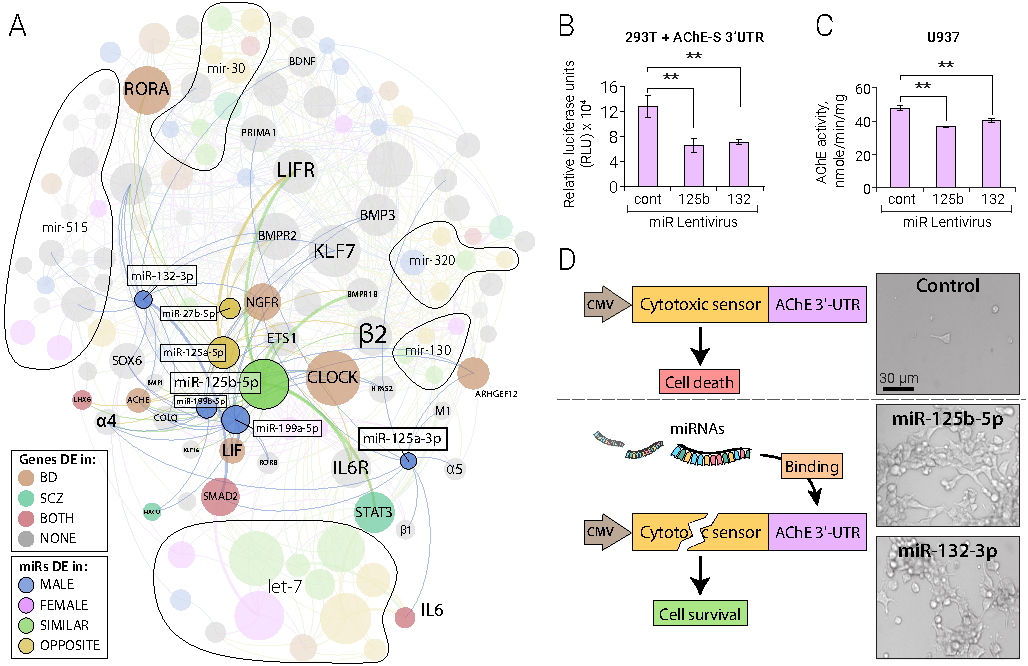
\includegraphics[width=\textwidth]{figures/smallnet}
\caption[The cholinergic/neurokine interface.]{\textbf{The cholinergic/neurokine interface.} \textbf{A)} The miRNA families mir-10 and mir-199 pose a sexually dimorphic interface of cholinergic, neurokine, and circadian regulation by targeting nicotinic/ muscarinic (e.g., a4b2 and M1) and neurokine receptors, transcriptional regulators of cholinergic differentiation (LHX and STAT) and circadian rhythm (CLOCK and RORA), the AChE and the AChE linker proteins PRIMA1/COLQ, and high-affinity choline uptake (HACU). Members of mir-10/199 families, spike-in miR-132-3p, and their targeted genes are shown in colour, and other miRNA families that passed the multiple filtering are indicated as areas. miRNA node size corresponds to count-change and gene node size to connectivity; colour and thicker edges indicate the DE context and experimentally validated connections. \textbf{B–D} Validation experiments of AChE targeting by miR-125b-5p, with miR-132-3p as a positive control. \textbf{B)} Lentiviral expression of miR-132 and miR-125b suppresses luciferase fused to the 3' UTR of AChE in HEK293T cells. Error bars indicate SE. \textbf{C)} Lentiviral expression of miR-132 and miR-125b suppresses the endogenous AChE hydrolytic activity of U937 cells with similar efficacy. Error bars indicate SE. \textbf{D)} Life/death assay of stably transfected HEK293T cells carrying the AChE 3' UTR fused to a cytotoxic sensor and co-transfected with miR-125b-5p, miR-132-3p, or control plasmids. Cells survive in case of binding of miR-132-3p and miR-125-5p to the 3' UTR.
\label{fig:smallnet}}
\end{figure}

In agreement with their localisation in the comprehensive network, miRNA families mir-10 and mir-199 inhabit a central role in the resulting interactome. Most-targeted genes in this network (as indicated by their size) are the circadian regulators CLOCK and \acs{rora}. While CLOCK is located centrally, next to mir-10/199 miRNAs, RORA shows closeness to the mir-30/515 families. Generally, genes with larger cellular influence, such as transcription factors (STAT3, CLOCK) or \ac{tgf}-$\upbeta$ ligands (BMP family genes) are frequently targeted by miRNAs, while more specific transcripts, such as the cholinergic receptor genes or neurokines, are targeted more selectively. \todo{more details?}

More so than the spiked-in miR-132-3p, mir-10/199 miRNAs target cholinergic genes, for instance, the neuronal nicotinic $\upalpha4\upbeta2$ and muscarinic M1 receptors (mir-125) and HACU (miR-199). In addition, they target neurokine genes, such as the transmembrane neurokine receptor LIFR or STAT3, and circadian regulators (e.g., CLOCK and RORA). The two families react highly sexually dimorphic to CNTF-mediated differentiation; some are detected as \ac{de} only in one cell line, others exhibit inverted changes between cell lines. The 3p-variant of miR-125a distinguishes itself from the bulk of mir-10/199 miRNAs by exclusively targeting M1, $\upalpha5$ and $\upbeta1$ receptors, and IL-6, and thus is slightly removed from the centre of the network. \todo{Describe other members?}

The miRNA with most targets in this reduced interactome is miR-125b-5p, also displaying most experimentally validated interactions with neurokine genes (miRTarBase accessions: IL-6, MIRT\-022105; IL-6R, MIRT006844; JAK2, MIRT734987; LIF, MIRT001037; LIFR, MIRT732494; \linebreak STAT3, MIRT005006). miR-125b-5p also is the most perturbed miRNA (in this interactome) upon CNTF-mediated differentiation (highest count-change), and the only member of mir-10/mir-199 to be changed in similar direction in both cell lines (up-regulated). miR-125b-5p also targets multiple other inflammation-related genes (e.g., \ac{tnf}, MIRT733472; IRF4, MIRT004534) and 5-lipoxygenase, which can influence inflammatory processes via production of eicosanoids.\cite{Busch2015} miR-125b-5b has been directly associated with cytokine-mediated inflammation, as its over-expression increased the expression of \ac{tnf}-$\upalpha$, IL-1$\upbeta$, and IL-6, and markedly decreased I$\upkappa$B-$\upalpha$.\cite{Zhang2017}

A notable intersection of spike-in miR-132-3p and miR-125b-5p is the \ac{ache}, an interaction which had not been validated for miR-125b-5p, but is known for miR-132-3p.\cite{Shaked2009, Shaltiel2013} Using miR-132-3p as a positive control, we performed ACHE-mRNA binding assays in validation of the predicted targeting by miR-125b-5p.

\begin{method}

\subsection{miR-125b-5p Acetylcholinesterase Targeting Assays}
We performed three independent cell culture assays to confirm \emph{ACHE} mRNA targeting by hsa-miR-125b-5p: luciferase suppression, AChE protein activity, and a cell death assay with a cytotoxic sensor. The 3' UTR of human \emph{ACHE} mRNA\cite{Soreq1990} was cloned into the microRNA Target Selection System plasmid (System Biosciences, CA, USA) multiple cloning site, using EcoRI and NotI restriction enzymes (New England Biolabs). All plasmids were verified by DNA sequencing. For luciferase assays, HEK293T cells were transfected with miRNA Target Selection-AChE-3' UTR, and selected in the presence of Puromycin for 3 weeks. Stably transfected HEK293T (293T-AChE 3' UTR) cells were grown on 12-well plates and infected with lentiviruses expressing miR-125b-5p, miR-132-3p or a negative control sequence. After 48 hours incubation, cells were analysed using the Dual Luciferase Assay kit (Promega, WI USA) and Luciferase activity was measured using an Envision luminescent plate reader (Perkin-Elmer, Waltham, MA), essentially as previously described by Hanin \emph{et al.}\cite{Hanin2014} For each reporter construct, renilla luciferase activity was normalized according to that of the firefly. Normalised activity after infection with miR-132-3p or miR-125b-5p was expressed as relative to that obtained after infection with the same plasmid with miRNA negative control. To show effects of changes in this miRNA’s levels on real-life protein activities, we performed an AChE hydrolytic activity assay following infection of human monocyte-like U937 cells with hsa-miR-125b-5p, miR-132-3p or a negative control lentiviral vector. AChE hydrolytic activity levels were assessed by kinetic measurements of the hydrolysis rates of \SI{1}{\milli\Molar} acetylthiocholine (ATCh, Sigma) at room temperature, following 20 min incubation with and without \SI{50}{\micro\Molar} tetraisopropyl pyrophosphoramide (iso-OMPA, Sigma), a specific inhibitor of butyrylcholinesterase, to selectively assay for AChE-specific or total cholinesterase activity. For the life/death assay, stably transfected HEK293T cells were infected with lentiviruses expressing miR-125b-5p, miR-132-3p or a negative control sequence. 72 hours post-infection, a cytotoxic reporter fused to AChE 3' -UTR was added to the media and cells were kept for an additional 5 days to assess their viability. For all cell culture assays, statistical significance was determined using ANOVA with correction for multiple testing. Each sample was assayed in at least 3 biological replicates, and in all cases, hsa-miR- 132-3p served as a positive control.

\end{method}

\subsection{hsa-miR-125b-5p Targets Acetylcholinesterase}
In all tested conditions, miR-125b-5p suppressed \emph{ACHE} mRNA with equal potency as the positive control miR-132-3p (Fig.\,\ref{fig:smallnet}\,B-D). Towards mRNA expression (luciferase) and functionality (cytotoxic sensor) as well as on protein level (AChE activity), miR-125b-5p demonstrated its interaction with ACHE mRNA 3' UTR. Luciferase units after miR-125b-5p transfection were approximately halved, indicating significant transcript degradation of the \emph{ACHE} 3'UTR.

\subsection{Cholinergic/Neurokine Mechanisms in Web-Available\\ RNA Sequencing Experiments}
To include recent developments in methodology, we analysed several recent \ac{seq} studies addressing related questions. In a study of post-mortem brain transcriptome profiling of psychiatric disorders,\cite{Ramaker2017} we found a down-regulation of IL-6, LIF, and several cholinergic receptors (M2, M4, $\upalpha$4, $\upbeta$2, $\upalpha$7), with sex-specific differences (males had significantly higher levels of neurokines than females). These changes were visible only in SCZ patients, not in BD or major depressive disorder. In a study of \acp{ipsc} of SCZ patients and controls that were induced to show a neuronal phenotype,\cite{Hoffman2017} we found an up-regulation of \emph{CHAT} in SCZ-derived iPSCs, and a down-regulation of IL6R and the nicotinic $\upalpha$6 subunit. In this study, SCZ males showed a higher expression of the \emph{SLC18A3} and lower expression of nicotinic subunits $\upalpha$ 2, 7, and 9, and $\upbeta$3. In a study of differentiated human neuronal progenitor cells,\cite{Fontenot2017} a knockdown of the circadian transcriptional controller CLOCK resulted in up-regulation of LIF and simultaneous down-regulation of neurokine transmembrane receptors LIFR and IL6ST, accompanied by slight bi-directional changes in several cholinergic receptors.
